\section{The PDF Trust Chain \note{1.5pp}}
\label{sec:background} 
\label{sec:trust-chain}

\subsection{Trust Chains, Abstractly}

Let's define what we mean by ``PDF Trust Chain''.

The term \emph{Trust Chain} is used in multiple contexts, e.g.,
\emph{digital certificates}: a sequence of certificates signing certificates,
starting with a root certificate;
\emph{supply chain}: a product is no more reliable or secure as its
outsourced components;
\emph{trusted boot}: unless the bootloader is correct and non-malicious,
there can be no possibility of the operating system being the same;
\emph{software stacks}: upper layers are dependent upon lower layers (such as
system libraries) and vulnerabilities at the bottom affect all layers above.

The common idea is that we have layers/components that rely on lower
\textcolor{blue}{is "lower" the correct term? Or "prior processing" and then "subsequent processing"?}
layers/sub-components/etc for their validity.
And the key lesson being,
{\bf{if a single element of the trust chain 
  is flawed or suborned, then every element ``above'' it
  is no longer capable of being trusted.}}


\subsection{The Trust Chain of a PDF Parser}

% In \cref{sec:pdf-challenges}, we elaborated on the challenges of PDF.
% Parsing data-formats has a long history and many solutions ...
% Parsing formal languages also has a long history and many solutions ...
% PDF has aspects of both: this makes PDF challenging.
% But PDF ``parsing'' is not merely a matter of harder [difference of degree]
% but intrinsically more complex [a difference of kind!]:

\begin{figure}[t]
    \centering
    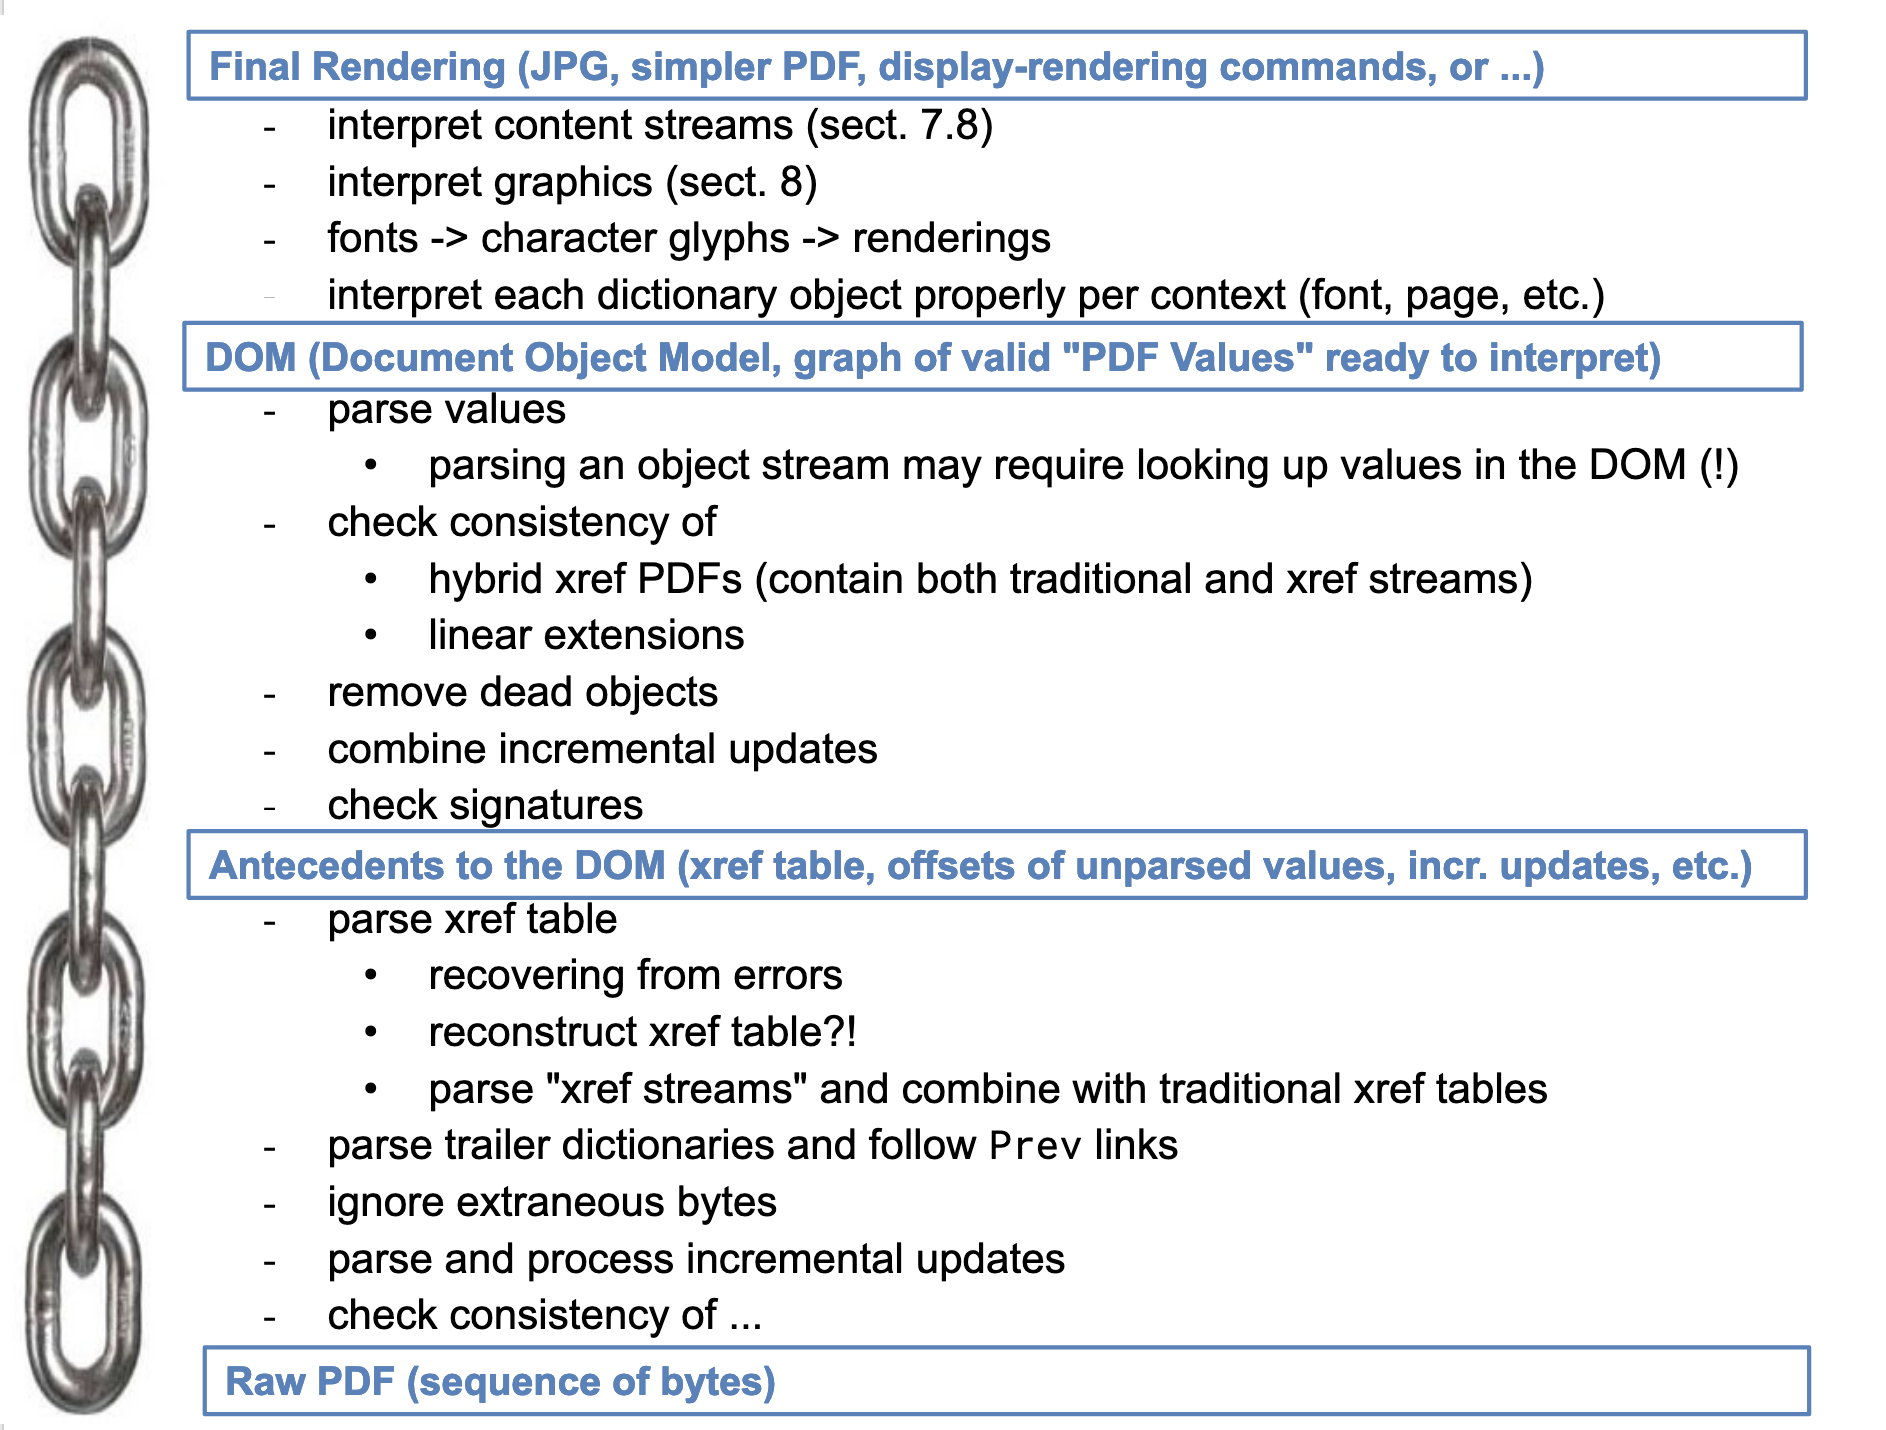
\includegraphics[width=0.8\linewidth]{figures/trustchain-diagram.png}
    \caption{The PDF Trust Chain diagrammed.}
    \todo{make diagram prettier!}
    \label{fig:pdf-trust-chain}
\end{figure}

In \cref{sec:pdf-challenges} we touched upon the complexities of parsing
PDF, but to appreciate these, one has to understand the
dependencies and interactions between the features.
In \cref{fig:pdf-trust-chain} we show the main components diagrammatically.
To briefly sketch what's going on here:
\begin{itemize}
\item Phase 1: we find the PDF header \verb|%PDF-x.y| (near start of the physical file, to account for preamble), then the end of the PDF file \verb|%%EOF| (near the end of the physical file), then "backwards parse" to find the last \verb|startxref| keyword followed by an end-of-line sequence and an integer value encoded as a sequence of ASCII bytes representing the byte offset in the PDF file (which is then adjusted for any preamble to a physical byte offset), and then locate either the \verb|xref| keyword for traditional PDF cross-reference tables, or a PDF object that should be a cross-reference stream. In the case of traditional PDF cross-reference tables, after the cross reference table will be the trailer dictionary identified by the \verb|trailer| keyword or, alternatively for PDF 1.5 and later files with cross-reference streams, the trailer dictionary keys will be in the stream extent dictionary of the cross reference stream. Of particular note is the \verb|Size| entry, which is one greater than the largest object number allocated in the PDF file. 
\item Phase 2: using information from Phase 1, we find and parse any incremental updates. These are identified by a \verb|Prev| entry in either the trailer dictionary or the stream extent dictionary of a cross-reference stream. The value of the \verb|Prev| key is another byte offset to the immediately preceding incremental update which, again, can either be a traditional cross-reference table and to the start of the \verb|xref| keyword, or to a cross-reference stream. This process  repeats, working from the most recent update back through time to the original PDF document.
\item Phase 3: data in each cross reference table must then be parsed to identify the byte offset to the start of each PDF object. Note also that PDF does not define the byte offset to the end of an object. There are two sets of objects in every PDF document: the in-use list of PDF objects and a free list of PDF objects. Object zero is always the start of the free list as it is not otherwise a valid object number. For incremental updates, PDF object numbering does not have to be sequential, with skipped object numbers assumed to be on the free list (although this is not stated explicitly in the PDF specification). Parsing depends on the form of the incremental update, with traditional cross-reference tables being simpler and larger independent of other processing. Cross-reference streams however are more complex as they are usually compressed and thus require the pre-DOM parser to "trust" the stream extent dictionary data.
\item Phase 4: using information from Phases 1, 2 and 3, the final set of objects that comprise the final PDF document can be established. Each incremental update can add new objects, mark existing in-use objects as free, or reinstate previously freed objects. \textcolor{blue}{do we want to mention the complexity of dig-sig here? what about cavities?} 
  \todo{More phases too?}
\item Phase 5: \todo{...} The result is the candidate DOM, 
  the candidate DOM is a mapping \lstcd{ObjId -> PdfValue}.
\item Phase 6: This phase takes the candidate DOM and verifies that
  it represents a sensible Document Tree per the PDF Standard.  E.g.,
  all indirect objects are in the candidate DOM, no unexpected recursion,
  etc.
\item Render Phase: we can now render the validated DOM, or parts thereof, to
  whatever display or graphic format we choose.
\end{itemize}

Note that phases 2, 3, 4 and 5
all require inputs from the previous phase to enable them to know where and
how to parse further segments of the PDF input file.
%
Note this: an implementation \emph{might} merge phases 1-4 into single phase
and give a \emph{semblance} of simplicity, but our argument (in what
follows in \cref{sec:specifying}) is that such an implementation will be
overly complex and we will have a near insurmountable task to assure that it
terminates for all input files.

% Only after Phase 5, have we correctly constructed a 'candidate' DOM (Document
% Object Model) where we have a mapping of Object Identifiers to PDF Values.

Although verifying Phase 5 is both difficult and tedious
(\todo{...; say something re the Arlington DOM model? Paper?})
and the Render phase has many complications of its own (fonts are
a special challenge, etc.), in this paper we focus on Phases 1-4.
We call these phases the pre-DOM parsing/computation, and if anything
goes wrong pre-DOM, lots can go wrong, the wrong DOM may be rendered, etc.!

\todo{Need to mention that validating a PDF with a digital signature entails identifying at which iteration of the PDF document the dig-sig was applied and then validating the dig-sig in the context of that specific DOM and the objects that were in effect at that instance in time.}

The attentive reader will note that we have another instance of a \emph{Trust
Chain}.  The later phases of the parsing process are \emph{completely
dependent} upon the earlier phases to properly parse and interpret the PDF
file.

% The PDF "trust chain": higher levels of abstraction depend upon lower levels.
% These structures are not necessarily concrete values--e.g. parsed xref
% table--but they do exist `conceptually'.


\textcolor{blue}{From the methodical process of trying to define the pre-DOM processing, it has been relatively easily to find Denial of Service attacks against various PDF implementations. e.g. multiple startxref very close together near EOF (failure of "backwards parsing"), Size is very large (either a DoS or "parser differential" without error), cyclic dependencies between Cross-reference and object streams (also a result of parsers not enforcing "must be direct" stated requirements)}


\todo{where do we want to mention ICC processing which has a simpler "Chain of Trust"? Should the text below not be PDF specific, but generic to file formats}

We think it is important to understand PDF parsing in terms of this
\emph{Trust Chain} as
%
(1) it highlights the presence of the many ``dependent'' parsers (or phases)
in PDF processing.
%
(2) it highlights the importance of ensuring the pre-DOM parsing, data integrity relationships and
computation (the base of our Trust Chain) is correct and secure.
%
(3) it reminds us that the integrity of the DOM cannot be verified
independently of the lower levels.

\todo{say ... regarding our repetitious use of ``parse and compute''}
\todo{we should use the concept of "data integrity relationships" being the essence of the necessary context. e.g. PDF incremental updates are appended to a previously valid PDF - thus an incremental update should not "make visible" a PDF object that was not already valid and visible in the original PDF (this is one method Shadow Attacks use - cf. an upstream "supply chain attack" by an attacker), even if that PDF object is otherwise entirely syntactically valid. In the same way an incremental update that refers to an object at a file byte offset after the incremental update would be highly suspicious.} 
\todo{ensure that spec.hs, the above text, and \cref{sec:specifying}
      are all consistent!}

